\section{Technical background}
PCPOP implements the monomials in partially-commutative monoid through the \emph{clique normal forms} and \emph{graph normal forms} as discussed in \cite{}. Here we briefly introduce and illustrate these normal forms.

Given a set of variables $X= \{x_1, x_2, \ldots, x_n\}$, and a graph $\graph=(X,E)$ with the vertices as the variables and the edge set capturing the commutation relations, i.e $(x_i,x_j) \in E$ if and only if $x_i$ and $x_j$ don't commute. This graph is called the independence graph. The dependence graph is the complement of the independence graph. To find the \emph{clique-normal form} $w^\clique$ for a word $w$, we project the word onto the maximal cliques of the dependence graph. This has been illustrated though the example below.
\begin{example}
Say $X=\{a,b,c\}$ and $[a,b] = [b,c]=0$ are the only commutations. The dependence graph is as shown below.
\begin{figure}[H]
\centering
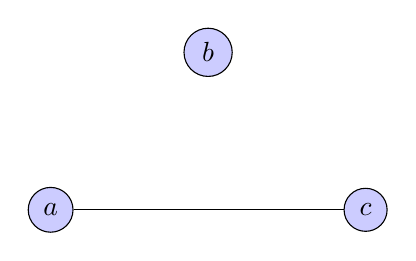
\begin{tikzpicture}
  \node[circle, draw, fill=blue!20] (a) at (0,0) {$a$};
  \node[circle, draw, fill=blue!20] (b) at (2,2) {$b$};
  \node[circle, draw, fill=blue!20] (c) at (4,0) {$c$};
  \draw (a) -- (c);
\end{tikzpicture}
\caption{Dependence graph}
\end{figure}
The maximal cliques are $\{b\}, \{a,c\}$. Now consider the words $w_1=c\mult a\mult b$ and $w_2=b \mult c \mult a$. The clique normal forms are $w^\clique_1 = w^\clique_2= ( c\mult a, b)$.
\end{example}

To compute the graph normal form of a word $w$, we label the different occurances of each letter in the word $w$ from left to right. For eg. for a word $w=a \mult b \mult a \mult c \mult b$, we label it as $a_1 \mult b_1 \mult a_2 \mult c_1 \mult b_2$. Then we build the directed graph $w^G$ whose vertices are the labeled letters and there is a directed edge $x \rightarrow y$ if the corresponding letters of the labels $x,y$ don't commute and if there is not path between them. It is illustrated as follows.
\begin{example}
Say $X=\{a,b,c\}$ and $[a,b] = [b,c]=0$ are the only commutations. Consider the word $w=a \mult b \mult a \mult c \mult b$. We label it as $a_1 \mult b_1 \mult a_2 \mult c_1 \mult b_2$. The graph $w^G$ is as shown below.
\begin{figure}[h!]
\centering
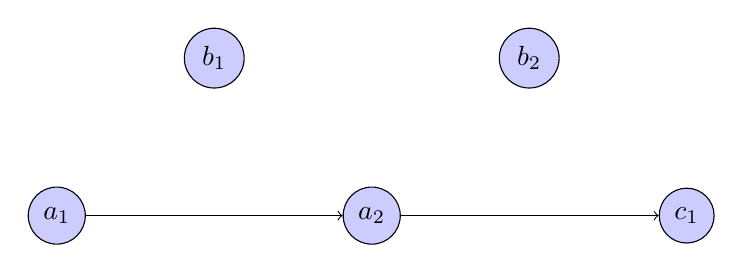
\begin{tikzpicture}
  \node[circle, draw, fill=blue!20] (a1) at (0,0) {$a_1$};
  \node[circle, draw, fill=blue!20] (b1) at (2,2) {$b_1$};
  \node[circle, draw, fill=blue!20] (a2) at (4,0) {$a_2$};
  \node[circle, draw, fill=blue!20] (b2) at (6,2) {$b_2$};
  \node[circle, draw, fill=blue!20] (c1) at (8,0) {$c_1$};
  \draw[->] (a1) -- (a2);
  \draw[->] (a2) -- (c1);
\end{tikzpicture}
\caption{Graph $w^G$}
\end{figure}
\end{example}
PCPOP handles special equality constraints like projectors, unitaries, dichotomic, orthogonality etc alongside partial commutations directly in the clique normal form. Although figure~\ref{fig:graph_product_multiplication} illustrates multiplication of graph product monomials, the mechanism to handle special equality constraints in partially commutative monomials is the same.


PCPOP also implements data structures to represent polynomials in graph product algebras and some new algorithms to find normal forms for certian type of graph product algebras and class of equality constriants[ see \cite{} for details]. A graph product algebra is the span of monomials belonging to a graph product monoid. Informally speaking, a graph product monoid is a monoid that combines different monoids where some monoids commute and some not. Partially-commutative monoid can be seen as special instance of grpah product algebra by repalcing the monoids with letters.

PCPOP implements the elements of partially commutative monoid and graph product monoid using same data structure called $\texttt{GraphProductWord\{V\}}$ where $V$ takes the type for variables when it partially-commutative word and type for monoid elements when it is a graph product word. The data structure $\texttt{GraphProductWord\{V\}}$ essentially consists of three fields, first being an array of array $\texttt{clique\_words}$ to hold the clique normal form and the other two are sets($\texttt{edge\_l,edge\_r}$) that hold the letters or monoid elements that can be commuted to the edge(left, right edge). Having the fields $\texttt{edge\_l, edge\_r}$ helps in efficiently implementing the multiplication of two graph product words. Below is an example, that illustrates how to find normal forms under partial commutations and projectors.
\begin{example}
Say we have two quantum systems  that belong to Alice and Bob respectively, Alice has two projective measurements $\{A_0,A_1\}$ and Bob has two projective measurements $\{B_0,B_1\}$ and there are two projectors $\{AB_0,AB_1\}$ that act on both Alice's and Bob's systems.  We know that Alice's and Bob's measurements commute with each other but not with the joint projectors. The operators belonging to Alice forms the free monoid $\monoid_A $, similarly, operators of Bob form $\monoid_B$ and the joint operators form $\monoid_{AB}$. We combine the monoids $\{\monoid_A,\monoid_B,\monoid_{AB}\}$ where $\monoid_A,\monoid_B$ commute to form the graph product monoid $\monoid$. Informally speaking, the maximal cliques are $\{\monoid_A,\monoid_{AB}\}$ and $\{\monoid_B,\monoid_{AB}\}$.

We can rewrite the words $w_1 = AB_0 \mult B_0 \mult A_1 \mult A_0$ and $w_2= A_1 \mult B_0 \mult AB_1$ as 

$w_1 = (AB_0)_{\monoid_{AB}} \mult (B_0)_{\monoid_B} \mult (A_1 \mult A_0)_{\monoid_A}$ and $w_2= (A_1)_{\monoid_A} \mult (B_0)_{\monoid_B} \mult (AB_1)_{\monoid_{AB}}$, where we multiply adjacent letters that belong to the same monoid and represented the result as word in respective monoid. 

Now If we multiply them, we get $w_1 \mult w_2 = (AB_0)_{\monoid_{AB}} \mult (B_0)_{\monoid_B} \mult (A_1 \mult A_0 \mult A_1)_{\monoid_A} \mult (AB_1)_{\monoid_{AB}}$, as $B_0$ can commute through $A_1$ and $A_0$.
In their clique normal forms, the multiplication algorithm is illustrated below.


\begin{figure}[H]
\centering
\label{fig:graph_product_multiplication}
\begin{tikzpicture}[scale=1]
  % w1 label above
  \node at (-5, 3) {$w_1$};
  % w1 as column vector
  \node at (-5, 2) {$\begin{bmatrix}(AB_0)(A_1 A_0)\\ \\(AB_0)(B_0)\end{bmatrix}$};
  % left-below set for w1
  \node at (-6.4, 1) {$\{\,AB_0\,\}$};
  % right-below set for w1
  \node at (-3.4, 1) {$\{\,(B_0),\ (A_1\,A_0)\,\}$};

  % multiplication symbol
  \node at (-1.3, 2) {$\times$};

  % w2 label above
  \node at (1.8, 3) {$w_2$};
  % w2 as column vector with two rows
  \node at (1.8, 2) {$\begin{bmatrix}(A_1)(AB_1)\\ \\(B_0)(AB_1)\end{bmatrix}$};

% left-below set for w2
  \node at (0.5, 1) {$\{\,(A_1),(B_0)\}$};
  % right-below set for w2
  \node at (3, 1) {$\{\,(AB_1)\}$};
  % equals symbol (centered under w1 and w2, moved further down)
  \node at (-1.2, 0.4) {$=$};

%%%%%%%%%%%%%%%%%%%%%%%%%%%%%%%%%%%%%%%%%%%%%%%%%%

    % w2 label above
  \node at (2.3, -0.3) {${w'}_2$};
    % w1 label above
  \node at (-5.5, -0.3) {${w'}_1$};
  \node at (-1.5, -0.3) {$m$};
  % w1' as column vector
  \node at (-5.5, -1.3) {$\begin{bmatrix}(AB_0)(A_1 A_0)\\ \\(AB_0)\end{bmatrix}$};
  % left-below set for w1'
  \node at (-6.9, -2.3) {$\{\,AB_0\,\}$};
  % right-below set for w1'
  \node at (-4.2, -2.3) {$\{\ (A_1\,A_0)\,\}$};

  % multiplication symbol
  \node at (-3.3, -1.3) {$\times$};
    \node at (-1.5, -1.3) {$\begin{bmatrix}\\ \\(B_0)\end{bmatrix}$};
    % left-below set for w1'
  \node at (-2.3, -2.3) {$\{(B_0)\}$};
  % right-below set for w1'
  \node at (-0.8, -2.3) {$\{(B_0)\}$};

\node at (0.3, -1.3) {$\times$};


  \node at (2.3, -1.3) {$\begin{bmatrix}(A_1)(AB_1)\\ \\(AB_1)\end{bmatrix}$};

% left-below set for w2'
  \node at (1.5, -2.3) {$\{\,(A_1),(AB_1)\}$};
  % right-below set for w2'
  \node at (3.8, -2.3) {$\{\,(AB_1)\}$};
  % equals symbol (centered under w1 and w2, moved further down)
  \node at (-1.1, -3) {$=$};
  % result as column vector (two rows) — moved up to reduce spacing from '='
  \node at (-1.1, -4.1) {$\begin{bmatrix}(AB_0)(A_1 A_0 A_1)(AB_1)\\ \\(AB_0)(B_0)(AB_1)\end{bmatrix}$};
  % result label just below its monomial representation — moved up accordingly
  \node at (-1.1, -5.1) {$w_1 * w_2$};
\end{tikzpicture}
\caption{Multiplication of graph product monomials (column vector view). Two words in their clique normal forms are multiplied. The clique normal forms are shown as column vectors(within square brackets) where each row has the projection of the word to the respective maximal clique. The words within simple brackets represent that they belong to a different monoids. The set below and left(right) to the clique normal forms represent the monoid elements that can be commuted to the left(right) edge. To multiply $w_1,w_2$ we check which monoid elements on the right edge of $w_1$ can be multiplied with the left edge elements of $w_2$. We represent the result of the multiplication in the middle as $m$. We update the clique normal forms and the left and right edge sets of $w_1,w_2$ accordingly to ${w'}_1^,{w'}_2$. We then multiply ${w'}_1*m*{w'}_2$ and we continue iteratively.}
\end{figure}  


\end{example}